\documentclass[11pt]{article}
\usepackage{float}
\usepackage{acl2014}
\usepackage{times}
\usepackage{url}
\usepackage{latexsym}
\usepackage{float}
\usepackage{graphicx} 
\usepackage{subfigure}

%\setlength\titlebox{5cm}

\title{Gender and Facial Expression Classification \\ (Intermediate project report)}

\author{Jifu Zhao\\
  Graduate Student\\
  Department of Nuclear, Plasma, and Radiological Engineering \\
  {\tt jzhao59@illinois.edu} \\}

\date{\today}

\begin{document}
\maketitle

\section{Project Review}
In this paper, the data is from FEI Face Database (Thomaz and Giraldi, 2010). There are 200 individuals including 100 males and 100 females. Both have two pictures with smile and non-smile expressions. So, this problem is basically a multiclass classification problem.

\section{Progress made}
After collecting the data, first they were correctly labelled manually into 4 classes-man smile, man non-smile, woman smile, and woman non-smile.\\

Then, using Python code, this original data set is randomly shuffled. And we select $75\%$ ($300$ faces) as the training set, and the rest $25\%$ ($100$ faces) as the test set.\\

In this question, the feature for three different pictures (frontal faces in gray scale, full faces in gray scale, colored faces) are as follows:
\begin{center}
$193 \times 162 = 31266$\\
$300 \times 250 = 75000$\\
$360 \times 260 \times 3 = 280800$\\
\end{center}

Based on the feature of the picture, a significant part of the original feature space is not useful for us. And if we do classification in the original feature space, we need large memory and powerful CPU. We don't want to waste resource on this, so our first step is to decrease the dimensionality. Here, we use Principal Component Analysis(PCA) method.\\

In PCA method, the first step is to center the data. After center the data, the mean faces are shown in Figure 1.

\begin{figure}[H]
\centering
\subfigure[frontal face]{
\label{Fig.sub.1}
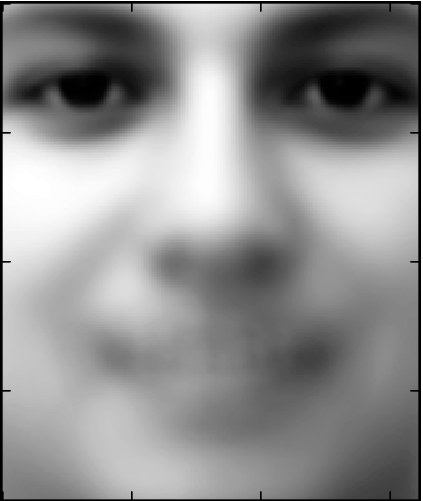
\includegraphics[width=20mm, height=25mm]{meanFace.png}}
\subfigure[full face]{
\label{Fig.sub.1}
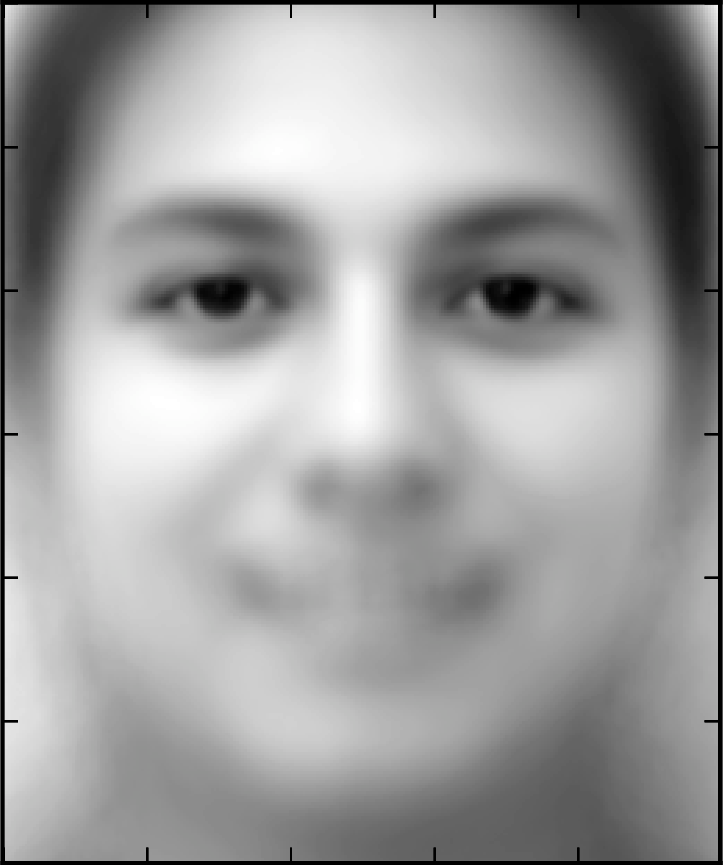
\includegraphics[width=20mm, height=25mm]{meanFace2.png}}
\subfigure[colored face]{
\label{Fig.sub.2}
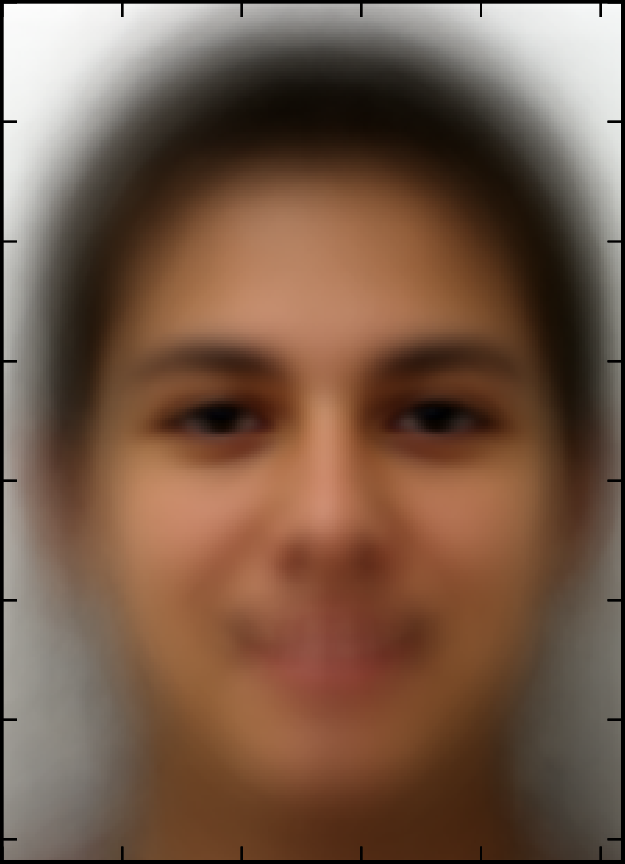
\includegraphics[width=20mm, height=25mm]{meanFace3.png}}
\caption{Mean faces}
\label{Fig1.lable}
\end{figure}

\begin{figure}[H]
\centering
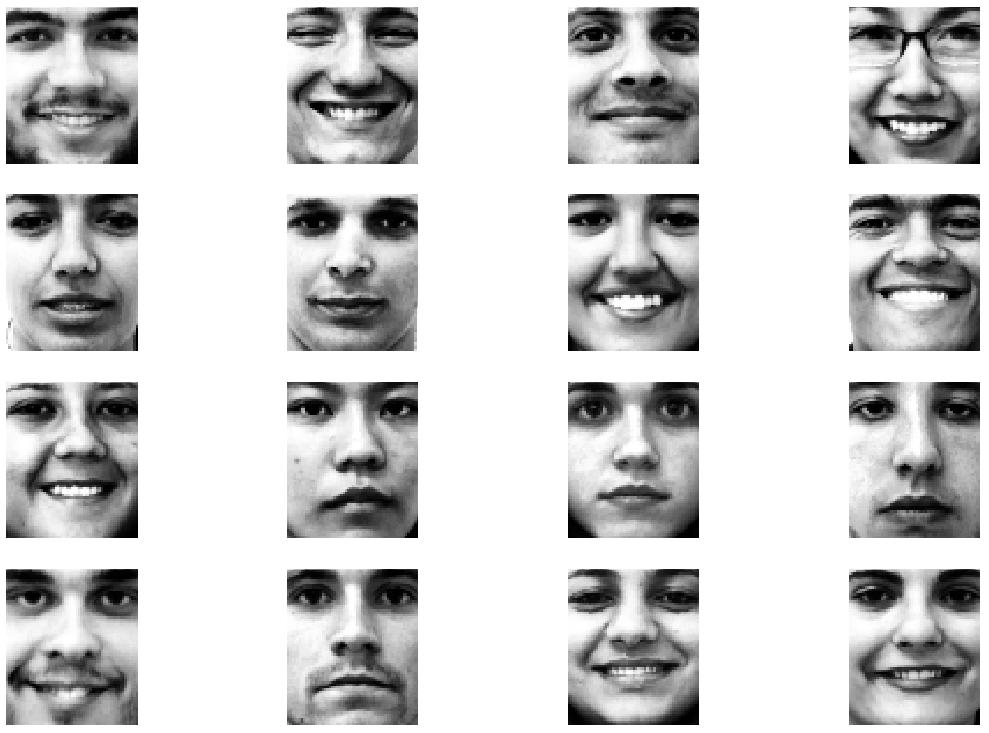
\includegraphics[width=80mm]{originalFace.png}
\caption{Original frontal faces}
\label{Fig2.lable}
\end{figure}

\begin{figure}[H]
\centering
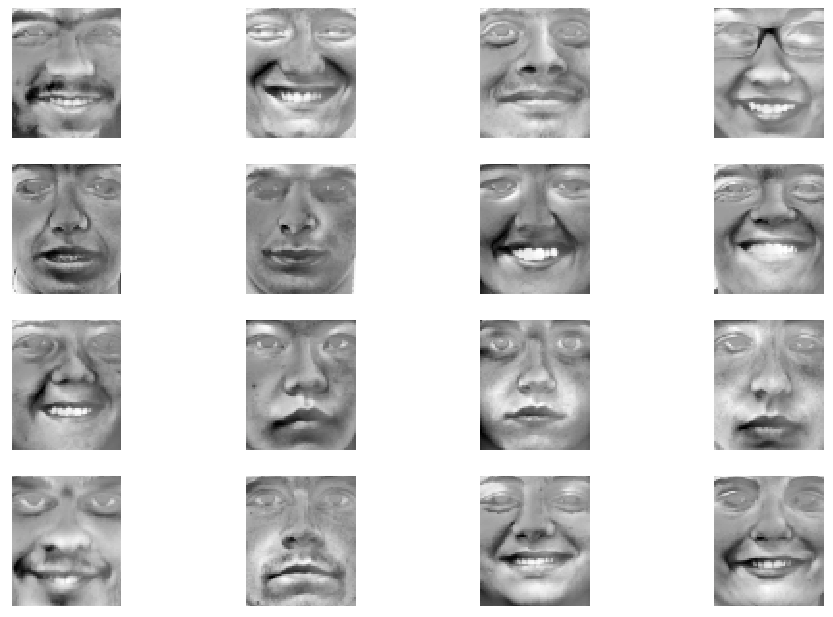
\includegraphics[width=80mm]{trainFace.png}
\caption{Centered frontal faces}
\label{Fig2.lable}
\end{figure}

After center the data, the original face will change a little bit. The original faces and centered faces are shown in Figure 2 and Figure 3 (Since the following analysis method are the same for three group figures, I will only show the result for {\bf frontal faces}).\\

Through PCA analysis, we can get a series of eigenvectors. In fact, there eigenvectors are the eigen-faces. They are shown in Figure 4.

\begin{figure}[H]
\centering
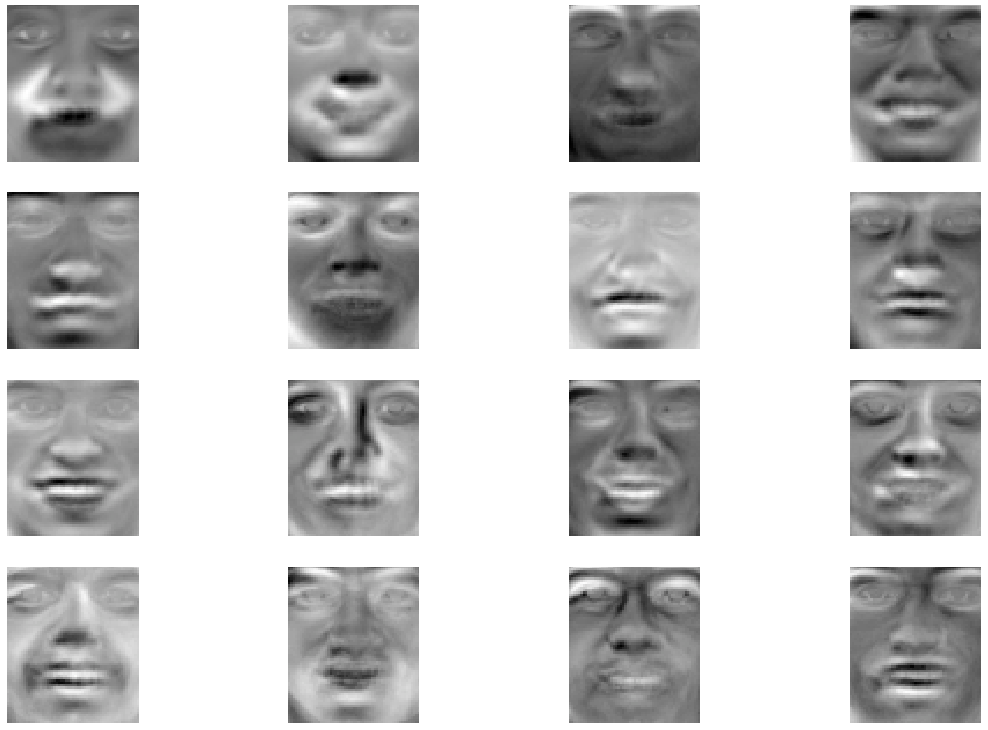
\includegraphics[width=80mm]{eigenFace.png}
\caption{Eigen frontal faces}
\label{Fig2.lable}
\end{figure}

The corresponding explained variance ratio, which measure the relative significance of the eigen faces, are shown in Figure 5

\begin{figure}[H]
\centering
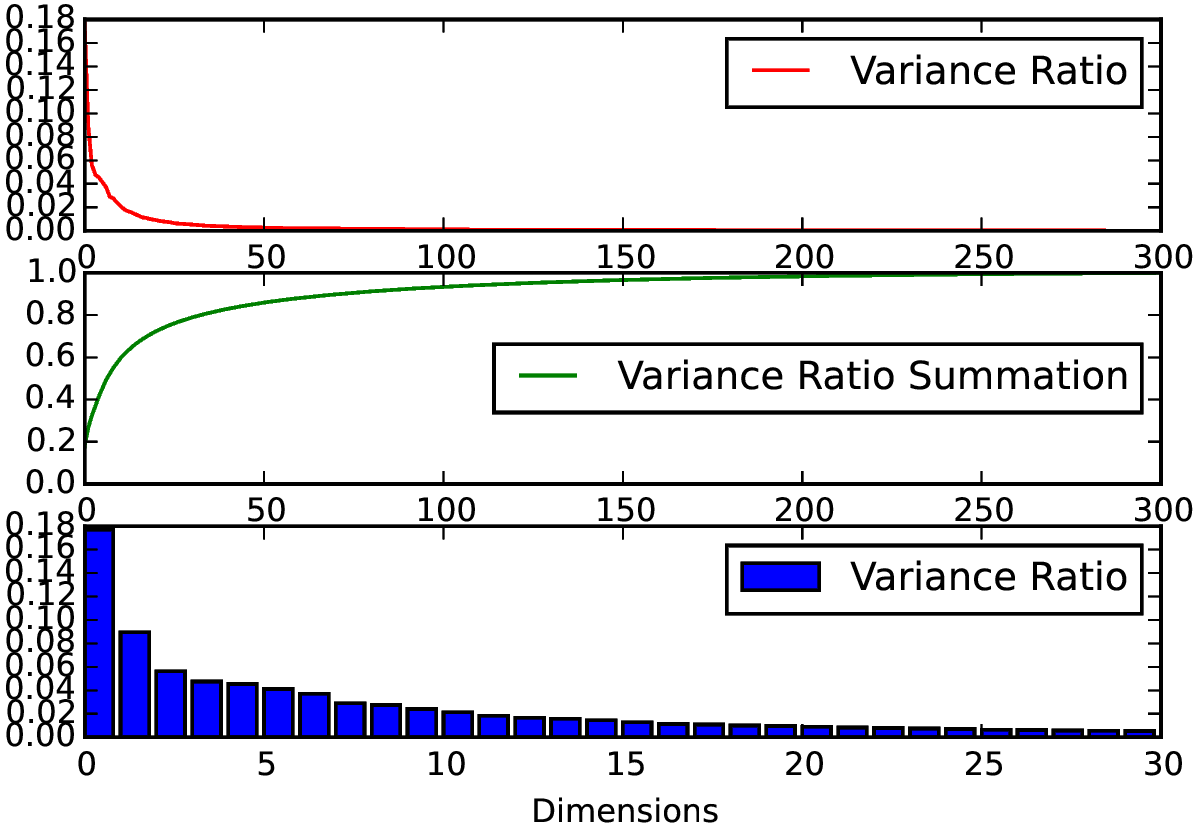
\includegraphics[width=70mm]{ratioChange.png}
\caption{Explained variance ratio}
\label{Fig2.lable}
\end{figure}

As, you can see from Figure 5, although there are originally $31266$ features, after PCA, 100 dimensions will include about $90\%$ changes. This means that our following analysis can based on the reduced feature space.\\

After PCA, we in fact got a series of eigenvectors, which stands for the eigen-faces. These eigen-faces can be used to reconstruct the original faces. This means that if we can maintain most of the information only use first several dimensions. For example, if we use only the first 2 dimensions and project the original faces onto these two eigenvectors, we can get the result shown in Figure 6.

\begin{figure}[H]
\centering
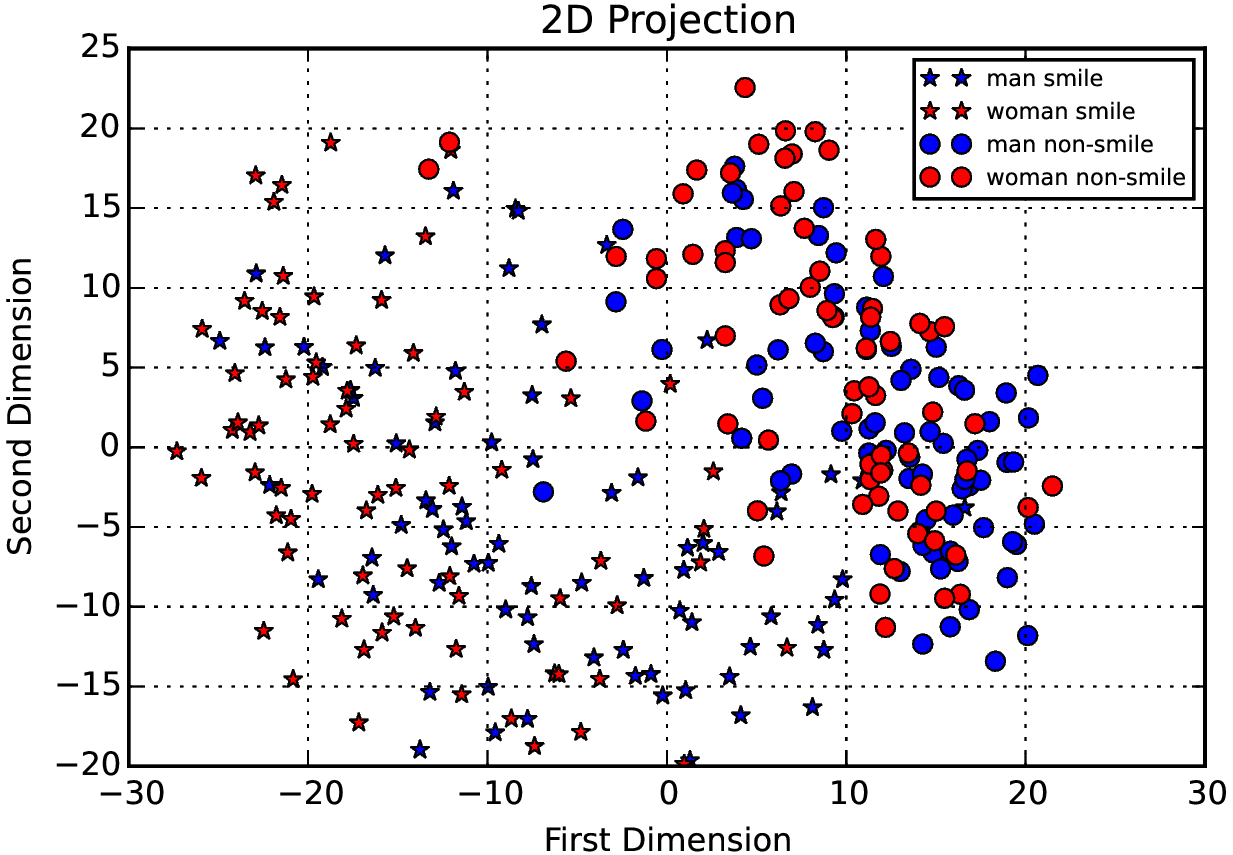
\includegraphics[width=90mm]{2dProjection.png}
\caption{2 dimension projection}
\label{Fig2.lable}
\end{figure}

As you can see in Figure 6, although smile and non-smile faces are not separated very well, man and woman faces have a relative very good separation. This is because that we only use the first 2 dimensions. The next step is to use more dimensions and try more algorithms on this problem.\\

\section{Plans}

Until now, I have successfully reduce the dimensionality from more than 30000 in to about 100 dimensions. The next step is to try some classification algorithms, such as support vector machines (SVM), Perception, Quadratic Discriminant Analysis and so on. Our goal is to quantitatively analyze this problem.\\

%\section{Changes}

\section{Difficulties}

Currently, the only problem is the data set problem. Now, we only have 400 faces. But we have more than 30000 features. This will influence the accuracy of our analysis. But we are still looking for more data.


\end{document}
